% English version of paper/ja_v3/04_解析.md (ver3 draft 2, 2026-11-17). The former RQ1(a) and RQ1(b) sections are merged into one analysis section (Ishii et al. 2022): a comparison subsection per question (what each numbered comparison verifies), then a results subsection whose subheadings name the comparisons and whose last paragraph gives the answer in one sentence. Interpretation and links to prior work are in the Discussion. The two-errors, distillation-flow and advantage figures and the table of the 11 methods moved to the Supplementary Information.
\FloatBarrier
\section{Analysis: which errors the information sources reduce, and when distillation raises UAR}\label{sec:analysis}

This section compares the conditions of groups A--C (Sect.~\ref{sec:conditions}) to analyse which part of the error each of the four information sources corrects (RQ1(a)) and which classifiers distillation improves, and when (RQ1(b)).

\subsection{Two parts of the error}\label{sec:twoerrors}
A linear classifier assigns an emotion using, for each pair of emotions, a boundary in feature space whose direction is set by the weights and whose position is set by the intercepts (Fig.~S2). An error in which the boundary has the right direction but is shifted, so that predictions are biased towards one emotion, is the \emph{answer bias}; it disappears when only the intercepts are corrected. The error that remains after correcting the bias is the \emph{remaining error}; it shrinks only when the direction of the weights changes.

We quantify the two parts as follows. For the score $s_k(x)=w_k^\top x+b_k$ of emotion $k$, the decision between emotions $k$ and $l$ is the sign of $z_{kl}=(w_k-w_l)^\top x+(b_k-b_l)$. With mean $\hat\mu_k$ and variance $v_k$ of $z_{kl}$ over target test utterances of emotion $k$ (likewise for $l$) and $\sigma=\sqrt{(v_k+v_l)/2}$, we define
\begin{equation}
d_{kl}=\frac{\hat\mu_k-\hat\mu_l}{\sigma},\qquad o_{kl}=-\frac{\hat\mu_k+\hat\mu_l}{2\sigma},
\end{equation}
the separation of the two emotions on the decision axis and the offset of the boundary ($z_{kl}=0$) from the midpoint of their means. If $z_{kl}$ of both emotions is normal with equal variance, the pairwise accuracy is $A(d,o)=\tfrac12[\Phi(d/2-o)+\Phi(d/2+o)]$. With the separation $D^{*}$ along the linear discriminant direction of the labelled target utterances (Ledoit--Wolf shrinkage \cite{ledoit2004}), the pairwise loss splits as
\begin{equation}
A(D^{*},0)-A(d,o)=\underbrace{[A(D^{*},0)-A(d,0)]}_{\text{direction loss}}+\underbrace{[A(d,0)-A(d,o)]}_{\text{intercept loss}}.
\end{equation}
Changing only the intercepts shifts $z_{kl}$ equally for all utterances and moves only $o$; a shift $x\to x+\delta$ common to all emotions also moves only $o$, so subtracting each corpus's feature mean does not change the direction loss. $D^{*}$ is used only for evaluation and is not the largest separation over linear directions. When this equal-variance Gaussian approximation was checked on source-only classifiers of the single-source setting, it met the pre-set fit criterion (median approximation error below one third of the median loss) for the direction loss except for visual features, but not for the intercept loss (Supplementary Information S2), so answer bias is measured by UAR differences rather than by the approximation.

\subsection{Comparisons for RQ1(a)}\label{sec:rq1a-compare}
In group A (single-source setting, K = 5), the following comparisons separate what one source corpus and the K labels correct.
\begin{itemize}
\item \textbf{(A2) $-$ (A0):} the gain of adding the K labels to the source-only classifier (hereafter the merged gain).
\item \textbf{(A3) $-$ (A0) and (A4) $-$ (A0):} neither the intercept-only fix nor mean subtraction changes the direction loss (Sect.~\ref{sec:twoerrors}); the share of the merged gain that they obtain measures how much correcting answer bias alone obtains.
\item \textbf{(A5) $-$ (A4):} whether correcting intercepts on the K labels adds to mean subtraction.
\item \textbf{The ratio $d_T(K)/D^{*}$ of (A1)} (K = 1, 5, 10): how close the weight direction comes to that of $D^{*}$ when only the K labels are used (remaining error).
\end{itemize}
In group B (all-source setting), we measure whether (B1) and each of (B2)--(B9) reduce the direction loss, averaged over the six emotion pairs, relative to (B0). The provider and weighting of the pseudo-labels of (B1) were chosen per condition on provisional targets (mostly the product of the classifiers' probabilities), and all include the retrained classifier's own modality. (B1) is measured in 81 conditions (each classifier with audio, visual and text on three corpora and with audio and visual on five corpora; K = 0, 5, 25) and (B2)--(B9) in 210 conditions (single modality; K = 0, 5), so the two counts do not compare the same conditions. Pre-set rules classified each condition as \emph{reduced}, \emph{same level}, \emph{increased} or \emph{undetermined} from the 95\% interval of the direction-loss difference ((B0) $-$ method) and an equivalence margin $\delta$ set from provisional-target outputs only (the full rules, the values of $\delta$, the hyperparameter selection and the intervals of groups A and B are in Supplementary Information S2). Some pseudo-label options (such as the product) were added after seeing results of an earlier version of the method on the same corpora.

\subsection{Results for RQ1(a)}

\subsubsection{Group A: the six conditions of the single-source setting}\label{sec:rq1a-single}
Table~\ref{tab:rq1a}(a) shows the group A differences by feature set. For audio and visual features, the intercept-only fix (A3) and mean subtraction (A4) obtained most of the merged gain. The summed (A3) gain was 0.78--0.91 times the summed merged gain. Label-free (A4) gained 4.69\pt\ [3.81, 5.57] for audio (WavLM) against the merged 5.26\pt, and 2.40\pt\ for visual against 2.47\pt. The interval of (A5) $-$ (A4) was not above zero for any of the eight feature sets (two audio, visual, text and four concatenations).

For (A1), which uses no source, $d_T/D^{*}$ (median over targets of the ratio averaged over six emotion pairs) was 0.23, 0.47 and 0.62 for audio (WavLM) at K = 1, 5 and 10, and 0.11, 0.32 and 0.42 for text. Visual reached 1.01 at K = 10 (the ratio can exceed 1 because $D^{*}$ is not the largest linear separation).

\begin{table}[!htbp]
\caption{Results for RQ1(a). (a) Group A (single-source setting, K = 5): UAR differences in points on test utterances; values are pair means (each pair averaged over repetitions 0--9); ``Ratio'' is $\sum$((A3) $-$ (A0)) $/ \sum$((A2) $-$ (A0)) over pairs; the last column gives 95\% intervals. (b) Group B (all-source setting): numbers of conditions by verdict. Direction loss: reduced / same level / increased / undetermined; UAR (method $-$ (B0)): higher / same level / lower / undetermined. ``16 more'' are conditions in which the adaptation term of DANN or MME did not change predictions beyond seed variation (separate from the 48 undetermined). Visual direction losses come from features that failed the approximation check (Sect.~\ref{sec:twoerrors})}\label{tab:rq1a}
\footnotesize
\textit{(a) Group A}\par\smallskip
\begin{tabular}{@{}lrrrl@{}}
\toprule
Features & (A2) $-$ (A0) & (A4) $-$ (A0) & Ratio & (A5) $-$ (A4) \\
\midrule
Audio (WavLM) & +5.26 & +4.69 & 0.91 & +0.38 [$-$0.12, +0.88] \\
Audio (HuBERT) & +4.73 & +4.18 & 0.90 & +0.18 [$-$0.42, +0.77] \\
Visual & +2.47 & +2.40 & 0.78 & $-$0.39 [$-$0.78, +0.02] \\
\botrule
\end{tabular}\par\medskip
\textit{(b) Group B}\par\smallskip
\begin{tabular}{@{}lllrll@{}}
\toprule
Cond. & Modalities & Classifier & Conditions & Direction loss$^{a}$ & UAR \\
\midrule
(B1) & A, V, T (3 corpora) & Audio & 9 & 9/0/0/0 & 9/0/0/0 \\
 &  & Visual & 9 & 1/1/0/7 & 1/0/0/8 \\
 &  & Text & 9 & 5/0/1/3 & 4/0/0/5 \\
 &  & AVT & 9 & 6/1/0/2 & 5/2/0/2 \\
 & A, V (5 corpora) & Audio & 15 & 7/0/0/8 & 7/0/0/8 \\
 &  & Visual & 15 & 5/0/0/10 & 4/1/0/10 \\
 &  & AV & 15 & 5/5/0/5 & 2/2/0/11 \\
\midrule
(B1) total & & & 81 & 38/7/1/35 & 32/5/0/44 \\
(B2)--(B9) & Single modality & A, V, T & 210 & 7/60/79/48 (16 more) & --- \\
\botrule
\end{tabular}
\footnotetext{$^{a}$Halving $\delta$ gives 49 of 81 ``reduced'' conditions for (B1); doubling it gives 20}

\end{table}

\subsubsection{Group B: (B1) and (B2)--(B9) in the all-source setting}\label{sec:rq1a-all}
Table~\ref{tab:rq1a}(b) shows that (B1) reduced the direction loss in 38 of 81 conditions and increased it in one; its UAR was judged higher than (B0) (same rule) in 32 and lower in none. (B2)--(B9) reduced the direction loss in 7 of 210 conditions and increased it in 79. If the true differences were zero and conditions independent, the expected numbers of ``reduced'' conditions would be 2.02 and 5.25. Comparing point estimates on the same anchors and conditions (two modality groups, K = 0 and 5), (B1) reduced the direction loss more in 341 of 373 pairs (pairs are not independent).

\subsubsection{Summary of the results for RQ1(a)}
The answer to RQ1(a) is therefore as follows. With one source corpus, the K labels and the source mainly corrected answer bias for audio and visual features, and label-free mean subtraction almost corrected it as well. In the all-source setting, pseudo-labels including other modalities reduced the remaining error in 38 of 81 conditions, whereas same-modality unlabelled utterances reduced it in only 7 of 210.

\subsection{Comparisons for RQ1(b)}\label{sec:rq1b-compare}
Distillation (C1) in group C (LOCO setting) retrains each of the audio, visual and text classifiers and the AVT classifier. The pseudo-label $q_i$ of each candidate utterance is the \emph{product}: the audio, visual and text classifiers are retrained from the anchor on the K labels and on the probabilities that the AVT classifier of (C0) assigns to the candidates, and their three probabilities are multiplied per utterance and normalised (Fig.~S3). $q_i$ includes the prediction of the retrained classifier's own modality. The loss of the retrained linear classifier is the cross-entropy on the K labels plus the cross-entropy towards the pseudo-labels of the candidates (the pseudo-label probabilities are targets without temperature) plus L2 terms towards the anchor $(W_0,b_0)$:
\begin{equation}
\begin{split}
L(W,b)=\frac{1}{S}\Big[&a\sum_{i\in\mathcal{K}}-\log p(y_i\mid x_i)+\sum_{i\in\mathcal{U}}\sum_k g_{ik}\,(-\log p(k\mid x_i))\\
&+\frac{\|W-W_0\|^2}{2C'}+\frac{\|b-b_0\|^2}{2C_b}\Big],
\end{split}
\end{equation}
with $p(\cdot\mid x)=\mathrm{softmax}(Wx+b)$ and $g_{ik}=(\rho n/4)\,q_{ik}/\sum_{j\in\mathcal{U}}q_{jk}$, where $\mathcal{K}$ is the set of K labelled utterances, $\mathcal{U}$ is the set of all $n$ candidates (including $\mathcal{K}$) and $S$ is the sum of the loss weights. The pseudo-label weights sum to $\rho n/4$ for each emotion. This loss form was fixed before the evaluation run; five other loss forms, including the temperature loss of Albanie et al.\ \cite{hinton2015distilling,albanie2018}, are compared in Supplementary Information S4. $C'$ and $C_b$ are those of (C0); the pseudo-label weight $\rho$, the K-label multiplier $a$ and the exponents of each modality in the product were chosen on the mean UAR over provisional targets (Sect.~\ref{sec:settings}); when several points were within two standard errors of the best, the one closest to the untuned values ($\rho=1$, $a=1$, exponents (1, 1, 1)) was chosen (grids in Supplementary Information S4). In all 48 conditions with K = 5, 10 and 25, the selected values gave the same classifier as the untuned values, so the product of (C1) and (D0) multiplies the three probabilities with equal weights. The values were fixed and recorded in a version-controlled file before the single evaluation run. The authors inspected UARs and differences (without intervals) of (C1) and (C2)--(C12) during the evaluation run (AFEW, IEMOCAP) and before aggregation; aggregation scripts were fixed beforehand and not changed.

Group C provides three comparisons.
\begin{itemize}
\item \textbf{(C1) $-$ (C0)} (audio, visual, text, AVT; K = 0, 5, 10, 25): which classifiers distillation improves.
\item \textbf{(C1) $-$ (C2)--(C12)} (K = 5, 10, 25): whether the gain of distillation can be obtained without pseudo-labels including other modalities. The 11 methods start from the same anchor and K labels and select hyperparameters by the same procedure. Because the encoders are frozen, DANN and MME are versions with their loss terms on a linear map and classifier, not the original methods that also train the feature extractor.
\item \textbf{Advantage and gain in (C13)} (K = 5, 25): how the gain of distillation relates to how often the pseudo-labels are correct.
\end{itemize}

(C13) consists of the retraining runs in which the evaluation run retrained each of the four classifiers on predictions of other classifiers instead of the product, with untuned $\rho=1$ and $a=1$. The providers are classifiers of (C0) (unimodal classifiers of other modalities, classifiers on two concatenated modalities, AVT), the product, the three classifiers that make the product, the AVT anchor and the classifiers of each source corpus. For each variant we measure (Fig.~S4):
\begin{itemize}
\item the \emph{advantage}: UAR of the provider's decisions $-$ UAR of the classifier before retraining, (C0), on candidates excluding the K labels, using candidate labels that are never used for retraining;
\item the \emph{gain}: UAR of the retrained classifier $-$ UAR of (C0) on test utterances.
\end{itemize}
K is 5 and 25, for which the candidate decisions of (C0) were saved. Excluding AVT retrained on its own predictions and duplicates of other providers leaves 360 variants per K (the excluded variants are in Supplementary Information S2; one of them, whose advantage is zero by construction, had a gain interval above zero). This is a descriptive analysis set up after the computation, without prior predictions; the authors had seen the gains and intervals of some providers before setting it up. Variants share candidates, test utterances and pseudo-label ingredients, so the rank correlations and counts below are not tests.

\subsection{Results for RQ1(b)}

\subsubsection{(C1) $-$ (C0): gain of distillation}\label{sec:rq1b-audio}
Table~\ref{tab:gain} shows (C1) $-$ (C0). Audio UAR after distillation was higher than that of (C0) in all 12 conditions with K = 5, 10 and 25 in point estimates, with intervals above zero in the nine conditions other than IEMOCAP (+2.71 to +4.15\pt). IEMOCAP gained +1.45 to +2.41\pt\ with intervals including zero at all three K. Without labels (K = 0), the audio gain had intervals above zero on all four corpora (+2.13 to +4.86\pt). The audio classifier retrained on pseudo-labels alone (K = 0) had higher UAR in point estimates than (C0) with 5 and 10 labels per emotion on all four corpora (values in Supplementary Information S2; no intervals computed).

The other classifiers gained less. Text gained +5.01 to +7.34\pt\ on IEMOCAP at K = 5, 10 and 25 with intervals above zero and had intervals including zero elsewhere; visual intervals were above zero only for MOSEI at K = 10 and 25, and AVT intervals only for MELD at all K and MOSEI at K = 25.

\begin{table}[!htbp]
\caption{(C1) $-$ (C0): gain of distillation (UAR points on test utterances) with 95\% intervals without correction. Values average 50 repetitions (5 for K = 0). At K = 0, (C0) is the anchor (source only) and (C1) uses no labels. K = 10 values follow an aggregation decided before the evaluation run (intervals only, no tests). IEMOCAP: improvised part}\label{tab:gain}
\footnotesize\setlength{\tabcolsep}{3.4pt}
\begin{tabular}{@{}lllll@{}}
\toprule
Corpus & K = 0 & K = 5 & K = 10 & K = 25 \\
\midrule
\multicolumn{5}{@{}l}{\textit{Audio}} \\
AFEW & +4.86 [+2.32, +7.40] & +4.15 [+2.56, +5.74] & +3.78 [+2.19, +5.38] & +3.32 [+1.40, +5.25] \\
IEMOCAP & +4.76 [+1.89, +7.63] & +2.41 [$-$0.45, +5.27] & +2.01 [$-$0.57, +4.58] & +1.45 [$-$0.48, +3.37] \\
MOSEI & +2.13 [+1.08, +3.19] & +3.19 [+2.38, +3.99] & +4.11 [+3.20, +5.01] & +3.36 [+2.56, +4.16] \\
MELD & +3.89 [+0.28, +7.51] & +3.12 [+1.18, +5.06] & +2.71 [+0.66, +4.77] & +2.86 [+1.21, +4.51] \\
\multicolumn{5}{@{}l}{\textit{Visual}} \\
AFEW & +2.48 [$-$1.34, +6.31] & +0.09 [$-$2.99, +3.17] & +0.18 [$-$1.90, +2.26] & $-$0.18 [$-$1.40, +1.04] \\
IEMOCAP & $-$2.08 [$-$5.19, +1.03] & $-$0.84 [$-$4.75, +3.06] & +0.91 [$-$4.76, +6.58] & $-$0.74 [$-$6.30, +4.82] \\
MOSEI & $-$0.91 [$-$2.35, +0.54] & +0.21 [$-$1.14, +1.56] & +1.56 [+0.16, +2.95] & +2.57 [+1.17, +3.98] \\
MELD & +0.67 [$-$2.76, +4.10] & +0.85 [$-$0.91, +2.61] & +0.71 [$-$0.50, +1.93] & +1.11 [$-$0.18, +2.40] \\
\multicolumn{5}{@{}l}{\textit{Text}} \\
AFEW & +1.56 [$-$2.33, +5.46] & +1.65 [$-$1.50, +4.79] & +1.83 [$-$0.92, +4.58] & +0.75 [$-$2.07, +3.56] \\
IEMOCAP & +7.52 [+4.75, +10.29] & +7.34 [+4.37, +10.31] & +6.87 [+3.06, +10.67] & +5.01 [+2.44, +7.57] \\
MOSEI & $-$0.69 [$-$1.72, +0.35] & $-$0.02 [$-$0.89, +0.84] & +0.79 [$-$0.02, +1.60] & +0.03 [$-$0.69, +0.74] \\
MELD & +0.18 [$-$2.56, +2.92] & $-$1.18 [$-$4.44, +2.08] & $-$1.28 [$-$3.15, +0.59] & $-$0.94 [$-$2.84, +0.95] \\
\multicolumn{5}{@{}l}{\textit{AVT}} \\
AFEW & +1.69 [$-$1.91, +5.30] & +1.03 [$-$0.65, +2.72] & +1.10 [$-$0.44, +2.65] & +0.62 [$-$0.33, +1.57] \\
IEMOCAP & +1.65 [$-$2.86, +6.16] & +0.16 [$-$4.53, +4.85] & +0.24 [$-$3.62, +4.09] & $-$0.83 [$-$5.12, +3.46] \\
MOSEI & $-$0.32 [$-$1.17, +0.54] & $-$0.35 [$-$0.90, +0.19] & +0.17 [$-$0.37, +0.70] & +0.74 [+0.18, +1.30] \\
MELD & +3.36 [+0.90, +5.81] & +2.53 [+1.65, +3.42] & +1.87 [+0.94, +2.80] & +1.41 [+0.63, +2.19] \\
\botrule
\end{tabular}
\end{table}

\subsubsection{(C1) $-$ (C2)--(C12): the 11 other methods}\label{sec:rq1b-methods}
For audio, (C1) $-$ method was positive in point estimates in all 132 comparisons over K = 5, 10 and 25, with intervals not above zero only in 10 comparisons on IEMOCAP (K = 5 UARs in Table~S2). (C7), which uses the classifier's own (C0) probabilities as pseudo-labels, gave $-$1.0 to +0.5\pt\ relative to (C0). For AVT the differences were mixed: some methods, such as self-training (C2) on AFEW (72.1 vs 70.8), were higher than (C1) in point estimates, and at K = 5 only CORAL (C9) on MOSEI was higher than (C1) with the interval of the difference below zero. The 11 methods use information other than pseudo-labels including other modalities, so we read these differences as differences in the information used rather than in the quality of the methods.

\subsubsection{(C13): advantage and gain}\label{sec:rq1b-margin}
For example, on MOSEI with K = 25, retraining the audio classifier on pseudo-labels from the visual--text classifier gave an advantage of +4.6\pt\ (42.2 vs 37.6) and a gain of +2.05 [+0.74, +3.35]\pt. On AFEW with K = 5, retraining the visual classifier on pseudo-labels from the audio--text classifier gave an advantage of $-$16.7\pt\ (54.4 vs 71.1) and a gain of $-$4.40 [$-$7.70, $-$1.09]\pt.

Over the 360 variants, the ranks of advantage and gain agreed: the rank correlation was 0.80 at K = 5 and 0.83 at K = 25, and within each of the 32 combinations of corpus, retrained classifier and K it was positive (median 0.92, minimum 0.39). Figure~\ref{fig:margincounts} counts the variants by the sign of the advantage and the gain interval. No variant with a negative advantage (173 at K = 5, 184 at K = 25) had a gain interval above zero, and 125 and 144 had intervals below zero. Among variants with a positive advantage (187 and 176), 58 and 42 had intervals above zero, while 16 and 20 had intervals below zero (breakdown in Supplementary Information S2).

\begin{figure}[t]
\centering
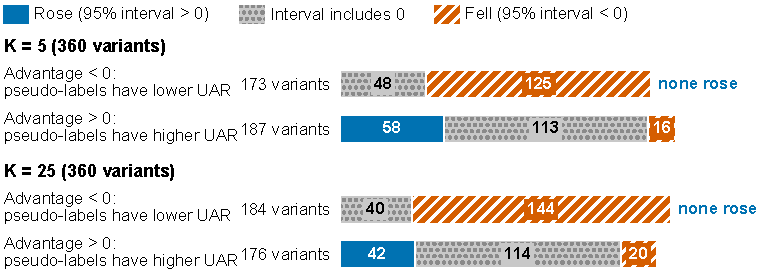
\includegraphics[width=\textwidth]{figures/fig_margin_counts_en.pdf}
\caption{Variants of (C13) (360 per K; K = 5 and 25) counted by the sign of the advantage and by the 95\% interval of the gain (above zero, including zero, below zero). One variant is one combination of corpus, retrained classifier and pseudo-label provider; the gain is the difference in test UAR. No variant with a negative advantage rose}\label{fig:margincounts}
\end{figure}

Among unimodal classifiers, the one whose (C0) had the highest candidate UAR (hereafter the corpus's strongest modality) was visual on AFEW, audio on IEMOCAP, visual on MOSEI and text on MELD at both K = 5 and 25. Retraining the classifier of the strongest modality on pseudo-labels from the classifier on the concatenated features of the other two modalities gave negative gains in point estimates in all eight cases (four corpora and two K; $-$4.40 to $-$1.02\pt).

\subsubsection{Summary of the results for RQ1(b)}
The answer to RQ1(b) is therefore as follows. Distillation gave higher audio UAR than (C0) in all 12 conditions in point estimates, with intervals above zero in the nine conditions other than IEMOCAP, and the gains of the visual, text and AVT classifiers varied in sign across corpora. Every (C13) variant whose UAR rose had pseudo-labels with higher UAR than the classifier before retraining.
